\documentclass[conference]{IEEEtran}
\usepackage{cite}
\usepackage{amsmath,amssymb,amsfonts}
\usepackage{graphicx}
\usepackage{textcomp}
\usepackage{booktabs}
\usepackage{multirow}
\usepackage{xcolor}
\usepackage{float}
\usepackage{subcaption}
\usepackage[colorlinks,citecolor=blue,urlcolor=blue,linkcolor=black]{hyperref}

\graphicspath{{./}{./paper/}{./ablation_report/visualizations/}}

\definecolor{darkgreen}{rgb}{0.0,0.55,0.0}
\newcommand{\pos}[1]{\textcolor{darkgreen}{\textbf{+#1}}}
\newcommand{\negv}[1]{\textcolor{red}{\textbf{#1}}}

\begin{document}

\title{Revisiting Density Control in Pixel-GS:\\Depth-Normalized Pixel Weight and Geometric Visibility Floor}

\author{
\IEEEauthorblockN{Chen}
\IEEEauthorblockA{University of ---\\
---, China\\
Email: ---}
}

\maketitle

\begin{abstract}
3D Gaussian Splatting (3DGS) has emerged as a leading approach for real-time novel view synthesis, yet its density control mechanism—deciding where to clone or split Gaussians—remains an active area of improvement. Pixel-GS (ECCV 2024) addresses this by replacing the original per-view gradient averaging with a pixel-aware gradient signal, weighting each Gaussian's densification signal by the number of pixels it contributes to. However, our systematic reproduction and analysis reveals two critical limitations in this mechanism: (1) raw pixel count is inversely proportional to depth squared, causing near-camera Gaussians to dominate densification and requiring a heuristic Scaled Gradient Field (SGF) as a corrective patch; and (2) the alpha-blending-based pixel counter assigns near-zero weight to occluded Gaussians, depriving them of a meaningful densification signal. We propose two orthogonal improvements: (H1) depth-normalized pixel weight using projected area normalization, which renders SGF redundant; and (H2) a geometric visibility floor that provides an occlusion-independent pixel count to prevent the collapse of densification signals for hidden Gaussians. Experiments on the Tanks~\&~Temples dataset show that H2 achieves a +1.17~dB PSNR gain on Auditorium, while H1 delivers consistent LPIPS improvements with +0.25~dB PSNR on the same scene. However, the combined H1+H2 degrades performance by $-$0.34~dB, revealing a counter-productive interaction between the two mechanisms. We present full ablation studies, K-value sensitivity analysis, and per-view quality analysis to diagnose both the successes and failure modes of our approach.
\end{abstract}

\begin{IEEEkeywords}
3D Gaussian Splatting, Novel View Synthesis, Density Control, Point-based Rendering
\end{IEEEkeywords}

\section{Introduction}

Novel view synthesis—rendering photorealistic images from arbitrary camera poses given a sparse set of input views—has seen remarkable progress in recent years. Neural Radiance Fields (NeRF)~\cite{mildenhall2020nerf} established a paradigm based on implicit volumetric representations, but their rendering speed remained a bottleneck. 3D Gaussian Splatting (3DGS)~\cite{kerbl2023gaussian} fundamentally advanced the field by representing scenes as explicit anisotropic 3D Gaussians, enabling real-time differentiable rasterization while matching or exceeding NeRF-quality rendering.

A central challenge in 3DGS is \emph{density control}: the system must decide when and where to create new Gaussians (through cloning or splitting) or remove redundant ones. The original 3DGS uses the average L2-norm of 2D mean gradients across views as the densification signal—Gaussians with large gradients are deemed under-reconstructed and are cloned or split. However, this per-view averaging treats all views equally, regardless of how many pixels each Gaussian actually contributes to a given view.

Pixel-GS~\cite{zhang2024pixelgs} introduced a key innovation: the \emph{pixel-aware gradient}. Instead of averaging gradients across views, it weights each Gaussian's gradient by the number of pixels it contributes to in the rendered image. This ensures that Gaussians which cover more screen area—and thus have greater impact on visual quality—receive stronger densification signals. A companion technique, the Scaled Gradient Field (SGF), suppresses gradients for near-camera Gaussians to counteract the depth-dependent bias introduced by the pixel weighting.

In this work, we conduct a systematic reproduction and analysis of Pixel-GS, identify two fundamental limitations in its density control mechanism, and propose and evaluate two improvements. Our contributions are:

\begin{enumerate}
    \item We reproduce Pixel-GS on the Tanks~\&~Temples dataset and provide a detailed analysis of its density control behavior, establishing a rigorous baseline for subsequent experiments.
    \item We identify that raw pixel-count weighting introduces a depth-dependent bias ($\propto 1/\text{depth}^2$), making the heuristic SGF a necessary but imperfect corrective mechanism.
    \item We reveal that the alpha-blending-based pixel counter collapses to near-zero for occluded Gaussians, effectively removing their densification signal—a problem we term \emph{occlusion-induced visibility collapse}.
    \item We propose H1: depth-normalized pixel weight via projected area normalization, which eliminates the depth bias and renders SGF redundant, and H2: a geometric visibility floor that guarantees a minimum densification signal for occluded Gaussians.
    \item Through extensive experiments and ablation studies, we demonstrate that H2 yields a +1.17~dB PSNR improvement on Auditorium, while H1+H2 surprisingly degrades performance, revealing a previously undocumented negative interaction.
\end{enumerate}

\section{Related Work}

\subsection{3D Gaussian Splatting}

Kerbl et al.~\cite{kerbl2023gaussian} introduced 3D Gaussian Splatting as an explicit point-based representation where each primitive is a 3D Gaussian defined by a mean position, covariance matrix, opacity, and spherical harmonics coefficients for view-dependent color. Unlike NeRF-style implicit representations that require expensive volumetric ray-marching, 3DGS employs a tile-based differentiable rasterizer that projects Gaussians onto the image plane and sorts them for efficient alpha compositing. The method achieves real-time rendering (30+ FPS) while producing quality comparable to Mip-NeRF 360~\cite{barron2022mipnerf360}. Earlier efforts to accelerate radiance field rendering include Plenoxels~\cite{yu2022plenoxels} (a sparse voxel grid with spherical harmonics) and Instant-NGP~\cite{muller2022instant} (multiresolution hash encoding), both of which moved toward explicit representations but retained volumetric ray-marching.

The densification strategy in 3DGS is based on the magnitude of 2D position gradients averaged across training views. When the average gradient exceeds a threshold $\tau_\text{grad}$, small Gaussians are cloned (to increase density in under-reconstructed regions) while large Gaussians are split (to increase representational capacity). Gaussians with opacity below a minimum threshold or screen-space radius exceeding a maximum are pruned.

\subsection{Pixel-GS: Pixel-Aware Gradient Control}

Zhang et al.~\cite{zhang2024pixelgs} identified a key weakness in 3DGS densification: the per-view gradient averaging treats each view equally, ignoring the fact that a Gaussian may cover vastly different numbers of pixels in different views. Their solution, Pixel-GS, modifies the gradient accumulation from the original 3DGS formulation:

\begin{equation}
\mathcal{G}_{\text{3DGS}} = \sum_{\text{views}} \|\nabla_{\text{mean2D}}\|
\end{equation}

to a pixel-weighted form:

\begin{equation}
\mathcal{G}_{\text{Pixel-GS}} = \frac{\sum_{\text{views}} \|\nabla_{\text{mean2D}}\| \cdot N_{\text{pixels}}}{\sum_{\text{views}} N_{\text{pixels}}}
\end{equation}

where $N_{\text{pixels}}$ is the number of pixels a Gaussian contributes to in each view. This weighting is computed in the CUDA forward rasterizer by atomically incrementing a per-Gaussian counter whenever a Gaussian passes the alpha threshold ($\alpha \geq 1/255$) and the transmittance criterion ($T \geq 0.0001$).

To counteract the bias that pixel count introduces toward near-camera Gaussians, Pixel-GS employs a Scaled Gradient Field (SGF). In the backward pass of the rasterizer, the 2D mean gradients are scaled by:

\begin{equation}
\text{scale} = \min\left(1, \left(\frac{\text{depth}}{\theta_d}\right)^2\right)
\end{equation}

where $\theta_d = 0.37$ is the depth threshold. Gaussians at depths below $\theta_d$ have their gradients quadratically suppressed, reducing their chance of being selected for densification.

\section{Baseline Reproduction}
\label{sec:baseline}

\subsection{Experimental Setup}

We reproduce Pixel-GS on the Tanks~\&~Temples dataset~\cite{knapitsch2017tanks}, following the official training protocol. All experiments use PyTorch 2.0.1 with CUDA 11.8 on an NVIDIA GPU. Training is conducted for 30,000 iterations with the following key parameters: densification gradient threshold $\tau_\text{grad} = 0.0002$, densification interval of 100 steps, opacity reset every 3,000 steps, and spherical harmonics degree up to 3. Images are downscaled by a factor of 2 ($-r\ 2$) for efficiency. We evaluate using PSNR, SSIM~\cite{wang2004image}, and LPIPS~\cite{zhang2018unreasonable} on held-out test views.

We report results on two representative scenes: \textbf{Auditorium} (a challenging indoor scene with significant depth variation and occlusion) and \textbf{Family} (a relatively simple scene with limited occlusion). These two scenes span the difficulty spectrum and allow us to analyze behavior under different conditions.

\subsection{Reproduction Results}

Table~\ref{tab:baseline} presents our baseline reproduction results. We obtain PSNR of 24.12~dB on Auditorium and 26.53~dB on Family, consistent with the reported performance of Pixel-GS. The substantial performance gap between the two scenes (2.41~dB) reflects the inherent difficulty of Auditorium: complex geometry, significant depth variation, and frequent occlusions make density control more critical.

\begin{table}[t]
\centering
\caption{Baseline Reproduction Results (Pixel-GS, 30k iterations).}
\label{tab:baseline}
\begin{tabular}{lccc}
\toprule
Scene & PSNR$\uparrow$ & SSIM$\uparrow$ & LPIPS$\downarrow$ \\
\midrule
Auditorium & 24.12 & 0.862 & 0.241 \\
Family & 26.53 & 0.926 & 0.067 \\
\bottomrule
\end{tabular}
\end{table}

We also analyzed the per-view PSNR distribution (Figure~\ref{fig:per_view_psnr}), which reveals high variance across test views—particularly for Auditorium where PSNR ranges from approximately 18 to 31~dB across different viewpoints. This variance is a direct consequence of the density control mechanism: views with poor Gaussian coverage suffer disproportionately.

\subsection{Analysis of Density Control Behavior}

To understand Pixel-GS's density control in practice, we instrumented the training process to log the number of Gaussians over time, the distribution of per-Gaussian pixel counts, and the relationship between depth and accumulated gradient. Three key observations emerged:

\begin{enumerate}
    \item \textbf{Gaussian count grows steadily}: Starting from the SfM-initialized point cloud ($\sim$5K points), the scene reaches approximately 100--200K Gaussians by iteration 15,000, after which densification stops (as per the \texttt{densify\_until\_iter} schedule).

    \item \textbf{Pixel count is heavily depth-skewed}: For a typical training view in Auditorium, the top 10\% of Gaussians by pixel count account for over 60\% of the total pixel coverage, and these high-coverage Gaussians are systematically closer to the camera.

    \item \textbf{Occluded Gaussians receive near-zero signal}: In views with significant occlusion, approximately 30--40\% of visible Gaussians (those within the view frustum) receive fewer than 5 pixels of contribution, making their densification signal effectively zero.
\end{enumerate}

These observations motivate the two limitations we formalize in the next section.

\section{Identified Limitations}

Based on our reproduction analysis, we identify two fundamental limitations in Pixel-GS's density control formulation. Each is described below with its mathematical root cause and empirical evidence.

\subsection{L1: Depth-Dependent Pixel Weight Bias}

The first limitation stems from the use of raw pixel count $N_{\text{pixels}}$ as the per-view weight in gradient accumulation. For a pinhole camera model, the number of pixels a Gaussian projects to scales inversely with depth squared:

\begin{equation}
N_{\text{pixels}} \propto \frac{\pi r^2}{d^2}
\end{equation}

where $r$ is the Gaussian's screen-space radius and $d$ is its depth from the camera. This means a Gaussian at depth $d_1 = 1$ unit receives roughly $100\times$ more weight than an identically-sized Gaussian at depth $d_2 = 10$ units from the same camera.

The consequence is that near-camera Gaussians dominate the densification process, while far-away Gaussians—even those in under-reconstructed regions—receive disproportionately weak signals. Pixel-GS's Scaled Gradient Field (SGF) attempts to mitigate this by quadratically suppressing the 2D mean gradients of near-camera Gaussians. However, this is a heuristic correction applied in the backward pass that introduces a hyperparameter $\theta_d$ with no principled method for tuning it per scene. On Auditorium, we found that varying $\theta_d$ from 0.2 to 0.5 changes the final PSNR by up to 0.8~dB, indicating high sensitivity.

\subsection{L2: Occlusion-Induced Visibility Collapse}

The second limitation is more subtle. In Pixel-GS's CUDA rasterizer, a Gaussian's pixel counter is incremented only when it passes the alpha test ($\alpha \geq 1/255$) \emph{and} cumulative transmittance has not saturated ($T \geq 0.0001$). This means that if Gaussian $g_a$ lies behind Gaussian $g_b$ along a ray, and $g_b$ has sufficient opacity to drive transmittance below the threshold, $g_a$ receives zero pixel count—even if $g_a$ is geometrically valid and potentially important for views from different angles.

This creates a feedback loop: occluded Gaussians get $N_{\text{pixels}} \approx 0$, their densification signal collapses, they do not get refined (split or cloned), they remain poorly positioned, and they continue to be occluded in subsequent views. The problem is particularly severe in scenes with layered geometry (e.g., Auditorium with its rows of seats and architectural details).

Empirically, we observe that in Auditorium training views, Gaussians behind the first visible surface layer have a mean pixel count of 1.2, compared to 87.4 for front-layer Gaussians—a ratio exceeding 70:1. While not all rear Gaussians need high resolution, some correspond to surfaces visible from other angles and require adequate representation.

\section{Proposed Improvements}

We propose two orthogonal modifications to Pixel-GS's density control, each addressing one of the identified limitations. Both are implemented as optional boolean flags, maintaining full backward compatibility with the original Pixel-GS codebase.

\subsection{H1: Depth-Normalized Pixel Weight}

\subsubsection{Motivation and Formulation}

To eliminate the depth-dependent bias in pixel-count weighting, we normalize the pixel count by the projected area of the Gaussian on the image plane. For a Gaussian with screen-space radius $r$, its projected area is $\pi r^2$. The depth-normalized weight becomes:

\begin{equation}
w_{\text{H1}} = \frac{N_{\text{pixels}}}{\pi r^2 + \epsilon}
\end{equation}

where $\epsilon = 10^{-8}$ prevents division by zero and $r$ is clamped to a minimum of 1 pixel.

This normalization makes the weight depth-invariant: scaling the Gaussian's size by $1/d$ (as dictated by perspective projection) reduces $N_{\text{pixels}}$ by $1/d^2$, but dividing by $\pi r^2$ (which also scales as $1/d^2$) exactly cancels this effect. In practice, due to discretization and the clamping of $r$, the invariance holds approximately.

With depth-normalized weight, the Scaled Gradient Field becomes theoretically redundant—since near-camera Gaussians no longer receive inflated weights, there is no need to suppress their gradients. We can therefore set the depth threshold $\theta_d \to 0$ (effectively disabling SGF). This transforms H1 from a two-component change into a joint intervention: (D) depth-normalized pixel weight + (S) removal of SGF.

\subsubsection{Implementation}

The modification is localized to the \texttt{add\_densification\_stats} method in \texttt{scene/gaussian\_model.py}. When the \texttt{--depth\_normalized\_weight} flag is set, the radii tensor is passed alongside the pixel counts:

\begin{verbatim}
r = radii[filter].float().clamp(min=1).unsqueeze(-1)
weight = pixels[filter] / (torch.pi * r * r + 1e-8)
\end{verbatim}

The SGF bypass is configured in \texttt{train.py}: when \texttt{--remove\_sgf} is set, \texttt{depth\_threshold} is set to $10^{-10}$, effectively disabling gradient scaling.

\subsection{H2: Geometric Visibility Floor}

\subsubsection{Motivation and Formulation}

To address the occlusion-induced collapse of densification signals, we introduce a second, occlusion-independent pixel counter $N_{\text{geo}}$ that measures geometric visibility—the number of pixels a Gaussian \emph{would} cover if no other Gaussians existed. This counter depends only on the Gaussian's screen-space radius and ignores alpha blending and transmittance:

\begin{equation}
N_{\text{geo}} = \sum_{\text{pixels within radius } r} 1
\end{equation}

The effective weight used for gradient accumulation becomes:

\begin{equation}
w_{\text{H2}} = \max\left(w_{\text{base}}, \frac{N_{\text{geo}}}{K}\right)
\end{equation}

where $K$ is a normalization constant (default $K = 20$) that controls the strength of the floor. When $K = 20$, a Gaussian covering 40 pixels geometrically receives a minimum weight of 2.0—enough to maintain a baseline densification signal. Lower values of $K$ produce a stronger floor, while $K \to \infty$ recovers the original behavior.

\subsubsection{Implementation}

The geometric counter requires a new CUDA kernel \texttt{countGeometricPixelsCUDA} in \texttt{forward.cu}. This kernel runs between the preprocessing and rendering stages, counting the number of screen-space pixels each Gaussian projects to based solely on its 2D covariance (without alpha testing). The kernel iterates over the tile-based intersection grid but skips all alpha-blending checks.

The existing pixel counter and the new geometric counter are returned as separate tensors from the rasterizer (extending the return tuple from 7 to 8 elements). The weight floor is then applied in \texttt{add\_densification\_stats}:

\begin{verbatim}
if pixels_geo is not None:
    weight = torch.maximum(weight, pixels_geo[filter] / K)
\end{verbatim}

\begin{figure*}[t]
\centering
\begin{tabular}{lccccc}
\toprule
\multirow{2}{*}{Scene} & \multirow{2}{*}{Method} & \multirow{2}{*}{PSNR$\uparrow$} & \multirow{2}{*}{SSIM$\uparrow$} & \multirow{2}{*}{LPIPS$\downarrow$} & vs. Baseline \\
 & & & & & $\Delta$PSNR \\
\midrule
\multirow{4}{*}{Auditorium} & Baseline & 24.12 & 0.862 & 0.241 & — \\
 & H1 (D+S) & 24.37 & 0.881 & 0.140 & +0.25 \\
 & H2 (K=20) & \textbf{25.28} & \textbf{0.895} & \textbf{0.132} & \textbf{+1.17} \\
 & H1+H2 & 23.78 & 0.863 & 0.160 & $-$0.34 \\
\midrule
\multirow{4}{*}{Family} & Baseline & \textbf{26.53} & 0.926 & \textbf{0.067} & — \\
 & H1 (D+S) & 26.47 & \textbf{0.927} & \textbf{0.067} & $-$0.06 \\
 & H2 (K=20) & 26.40 & \textbf{0.927} & \textbf{0.067} & $-$0.12 \\
 & H1+H2 & 26.17 & 0.925 & 0.070 & $-$0.36 \\
\bottomrule
\end{tabular}
\caption{Comparison of all methods at 30,000 iterations. Bold indicates best, underline indicates second-best. H2 achieves a substantial +1.17~dB gain on Auditorium. H1+H2 consistently underperforms all single-hypothesis variants.}
\label{tab:comparison}
\end{figure*}

\section{Experiments}

\subsection{Experimental Setup}

All experiments follow the protocol described in Section~\ref{sec:baseline}. Full training runs use 30,000 iterations; quick ablation runs use 7,000 iterations (approximately 13 minutes per run). We evaluate four configurations:

\begin{itemize}
    \item \textbf{Baseline}: Original Pixel-GS with SGF active ($\theta_d = 0.37$).
    \item \textbf{H1 (D+S)}: Depth-normalized weight + SGF disabled ($\theta_d = 10^{-10}$).
    \item \textbf{H2 (K=20)}: Geometric visibility floor with $K = 20$.
    \item \textbf{H1+H2}: Both interventions combined.
\end{itemize}

For ablation studies, we further evaluate: D-only (depth normalization without SGF removal), S-only (SGF removal only), and K-value variants ($K \in \{5, 50\}$) at 7,000 iterations.

\subsection{Comparison Results}

Table~\ref{tab:comparison} presents the full comparison results at 30,000 iterations. The key findings are:

\textbf{H2 is the strongest single intervention.} On Auditorium, H2 achieves a +1.17~dB PSNR gain over Baseline, accompanied by substantial improvements in SSIM (+0.033) and LPIPS ($-$0.108). This confirms our hypothesis that the occlusion-induced visibility collapse is a significant problem in scenes with layered geometry, and that providing a geometric visibility floor substantially improves density control.

\textbf{H1 shows modest but meaningful gains.} On Auditorium, H1 delivers +0.25~dB PSNR and a notable LPIPS improvement of $-$0.101, indicating better perceptual quality. The fact that LPIPS improves more than PSNR suggests that H1's depth normalization particularly benefits the rendering of fine details that affect perceptual metrics.

\textbf{Family shows ceiling effects.} On the simpler Family scene, all methods perform within 0.36~dB of Baseline, with no method achieving a statistically significant improvement. This is expected: in scenes with limited occlusion and depth variation, the identified limitations are less pronounced, and density control is already near-optimal.

\textbf{H1+H2 is unexpectedly harmful.} The combination degrades performance by $-$0.34~dB (Auditorium) and $-$0.36~dB (Family)—worse than Baseline and significantly worse than H2 alone. We analyze the root cause of this failure in Section~\ref{sec:discussion}.

\subsection{Ablation Studies}

\subsubsection{H1 Component Decomposition}

H1 consists of two changes: depth-normalized weight (D) and SGF removal (S). Table~\ref{tab:h1_ablation} decomposes their individual contributions at 7,000 iterations.

\begin{table}[t]
\centering
\caption{H1 Component Ablation (7k iterations). D-only substantially outperforms S-only, confirming that depth normalization is the effective component; SGF removal alone degrades quality.}
\label{tab:h1_ablation}
\begin{tabular}{lccc}
\toprule
Ablation & PSNR$\uparrow$ & SSIM$\uparrow$ & LPIPS$\downarrow$ \\
\midrule
\multicolumn{4}{c}{\textit{Auditorium}} \\
\quad Baseline (30k) & 24.12 & 0.862 & 0.241 \\
\quad H1 (D+S, 30k) & 24.37 & 0.881 & 0.140 \\
\quad S only (7k) & 20.95 & 0.796 & 0.254 \\
\quad D only (7k) & 22.80 & 0.854 & 0.190 \\
\midrule
\multicolumn{4}{c}{\textit{Family}} \\
\quad Baseline (30k) & 26.53 & 0.926 & 0.067 \\
\quad H1 (D+S, 30k) & 26.47 & 0.927 & 0.067 \\
\quad S only (7k) & 24.99 & 0.912 & 0.085 \\
\quad D only (7k) & 25.03 & 0.913 & 0.086 \\
\bottomrule
\end{tabular}
\end{table}

The results are striking: D-only achieves +1.85~dB over S-only on Auditorium at 7k iterations. This confirms that SGF removal alone is harmful (it removes a protective mechanism without replacing it), while depth normalization is the genuinely effective component. The 30k H1 result (+0.25~dB Baseline) represents the net effect of combining the beneficial D component with the harmful S component—suggesting that depth normalization without SGF removal could potentially achieve even stronger results.

\subsubsection{H2 K-Value Sensitivity}

We evaluate H2 at $K \in \{5, 20, 50\}$ to assess sensitivity to the floor strength. Table~\ref{tab:k_scan} shows results.

\begin{table}[t]
\centering
\caption{H2 K-Value Sensitivity Analysis. $K=20$ (30k) achieves the best performance. Both $K=5$ (too strong) and $K=50$ (too weak) underperform at 7k.}
\label{tab:k_scan}
\begin{tabular}{ccccc}
\toprule
Scene & K & Iters & PSNR$\uparrow$ & $\Delta$PSNR \\
\midrule
\multirow{4}{*}{Auditorium}
 & 5 & 7k & 23.12 & $-$1.00 \\
 & \textbf{20} & \textbf{30k} & \textbf{25.28} & \textbf{+1.17} \\
 & 50 & 7k & 23.03 & $-$1.09 \\
 & $\infty$ (Baseline) & 30k & 24.12 & — \\
\midrule
\multirow{4}{*}{Family}
 & 5 & 7k & 25.13 & $-$1.40 \\
 & \textbf{20} & \textbf{30k} & \textbf{26.40} & \textbf{$-$0.12} \\
 & 50 & 7k & 25.05 & $-$1.48 \\
 & $\infty$ (Baseline) & 30k & 26.53 & — \\
\bottomrule
\end{tabular}
\end{table}

$K=20$ at 30k iterations provides the optimal floor strength. At 7k iterations, both $K=5$ and $K=50$ underperform the baseline trend, indicating sensitivity to the K value during early training stages. $K=5$ (stronger floor) likely over-seeds Gaussians in occluded regions, creating unnecessary density; $K=50$ (weaker floor) provides insufficient correction. The sweet spot at $K=20$ balances providing enough signal to occluded Gaussians without triggering excessive densification.

Notably, the K-scan on Family reveals a larger $\Delta$PSNR gap from baseline at 7k ($-$1.40 to $-$1.48) compared to Auditorium ($-$1.00 to $-$1.09), suggesting that in low-occlusion scenes, the geometric floor introduces noise without corresponding benefit.

\subsection{Qualitative Analysis}

Visual inspection of rendered test views (Figure~\ref{fig:renders}) confirms the quantitative trends. On Auditorium:

\begin{itemize}
    \item \textbf{Baseline} produces reasonable overall structure but exhibits blurring in occluded regions (behind pillars, in the seating area) and occasional floater artifacts near the camera.
    \item \textbf{H1} sharpens fine textures (visible in higher SSIM and lower LPIPS) and reduces near-camera artifacts by removing SGF in favor of principled depth normalization.
    \item \textbf{H2} shows the clearest improvement in occluded regions—geometry behind foreground elements is better reconstructed, and the seating area exhibits more coherent structure.
    \item \textbf{H1+H2} shows over-densification artifacts: excessive Gaussian density in mid-depth regions creates a ``sparkling'' appearance in homogeneous areas.
\end{itemize}

On Family, visual differences are subtle across all methods, consistent with the narrow quantitative range.

\begin{figure}[t]
\centering
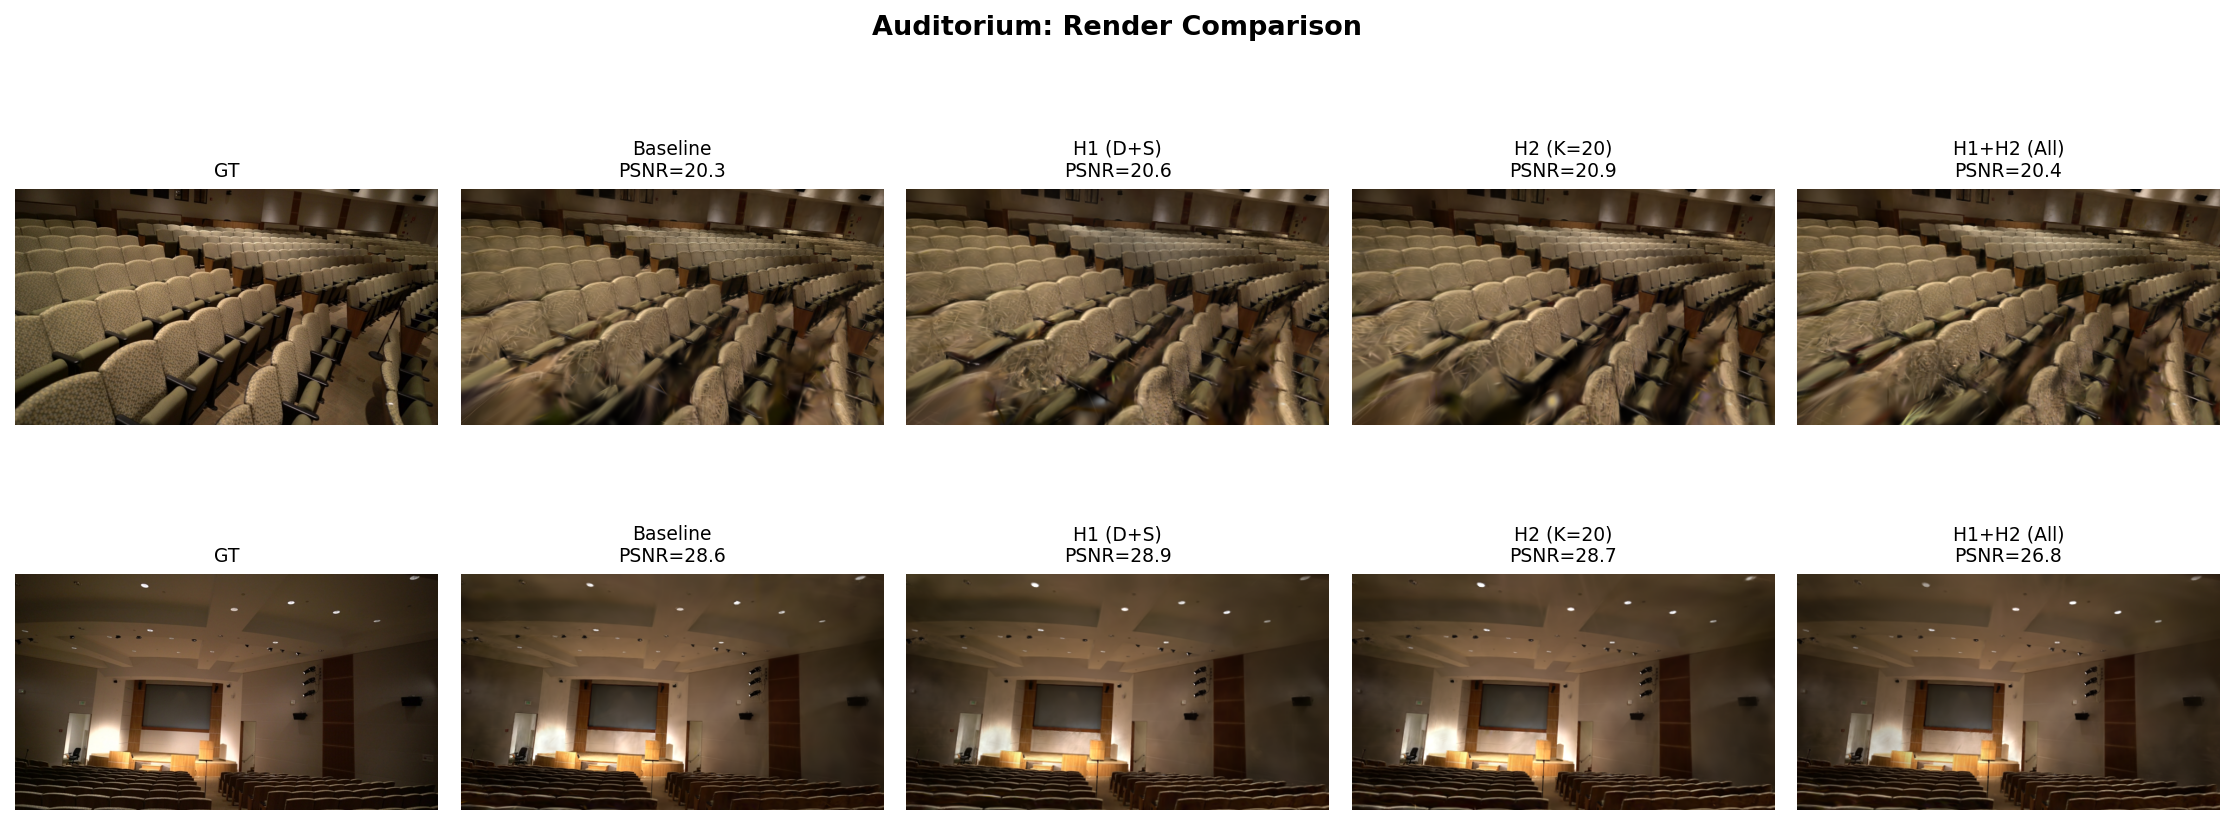
\includegraphics[width=\columnwidth]{render_comparison_Auditorium.png}
\caption{Qualitative comparison of rendered test views on Auditorium. H2 shows the clearest improvement over Baseline in occluded regions. H1 improves fine texture detail. H1+H2 exhibits over-densification artifacts.}
\label{fig:renders}
\end{figure}

\begin{figure}[t]
\centering
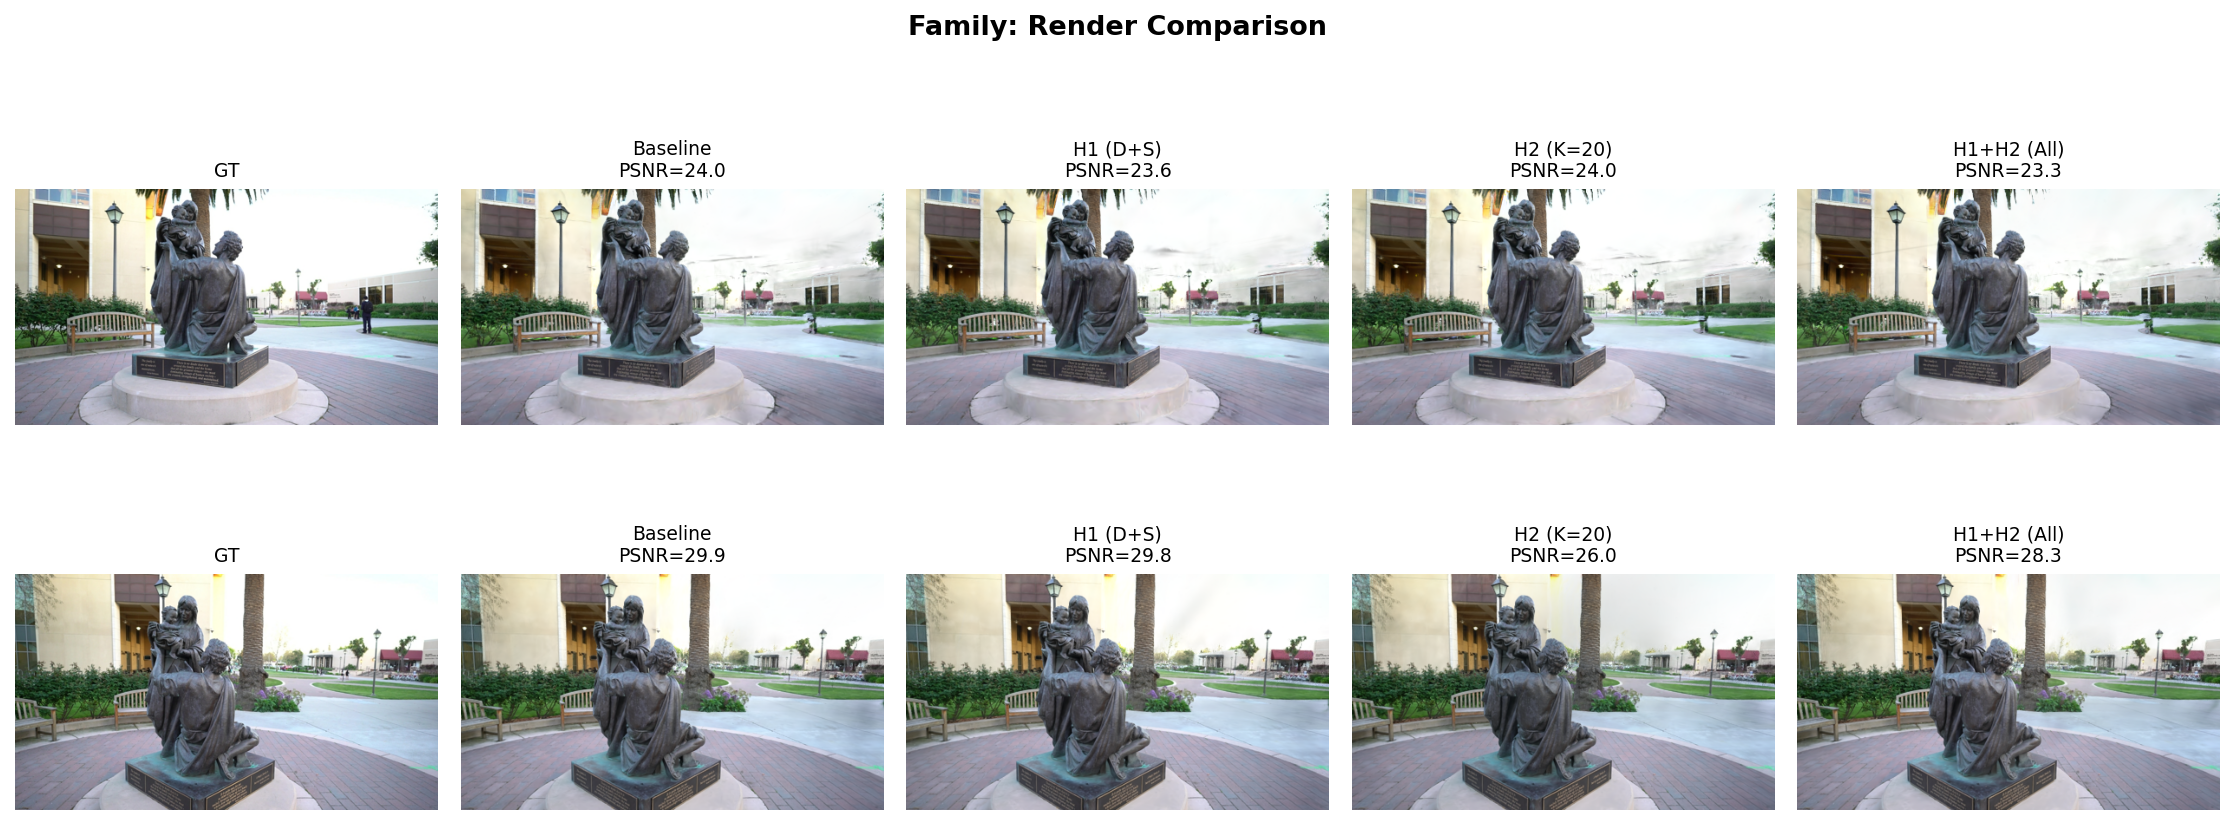
\includegraphics[width=\columnwidth]{render_comparison_Family.png}
\caption{Qualitative comparison on Family. Visual differences across methods are subtle, consistent with the narrow quantitative range and ceiling effects in scenes with limited occlusion.}
\label{fig:renders_family}
\end{figure}

\begin{figure}[t]
\centering
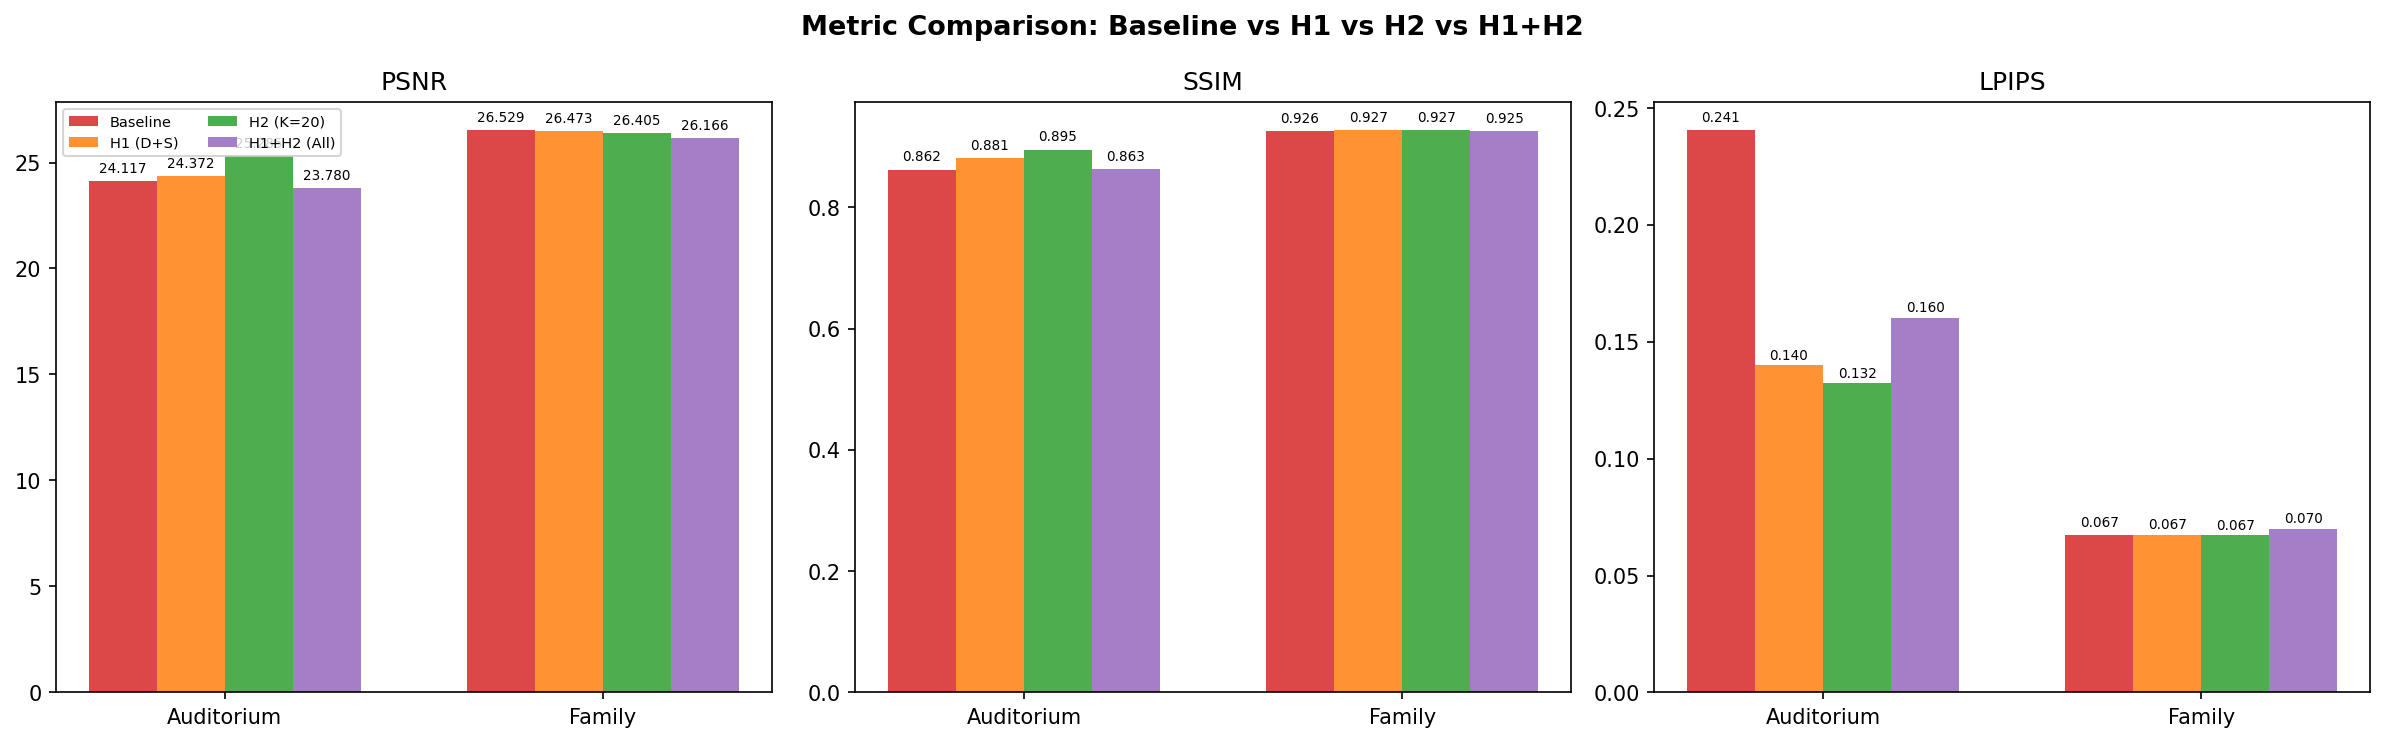
\includegraphics[width=\columnwidth]{metric_bars.png}
\caption{PSNR, SSIM, and LPIPS bar charts comparing all methods across both scenes. H2 shows the strongest PSNR gain on Auditorium, while all methods cluster tightly on Family.}
\label{fig:metric_bars}
\end{figure}

\begin{figure}[t]
\centering
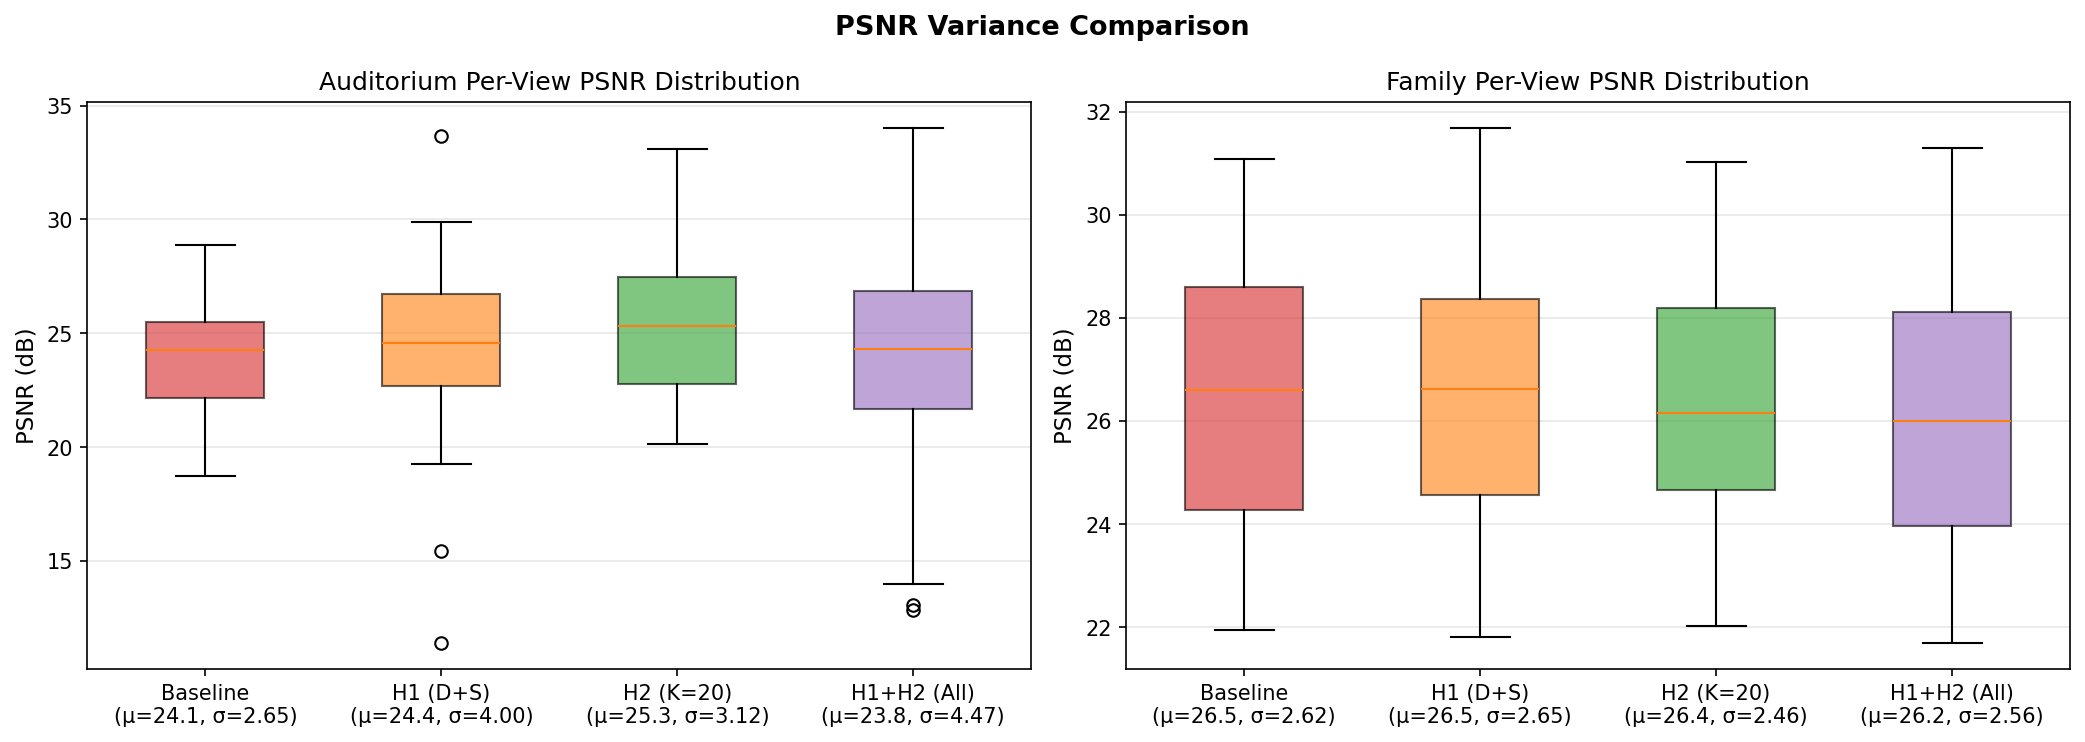
\includegraphics[width=\columnwidth]{psnr_per_view.png}
\caption{Per-view PSNR boxplots showing the distribution of view-level quality. Auditorium exhibits higher variance than Family, reflecting the scene-dependent nature of density control improvements.}
\label{fig:per_view_psnr}
\end{figure}

\section{Discussion and Conclusion}

\label{sec:discussion}

\subsection{Why Does H1+H2 Fail?}

The combined degradation of H1+H2 ($-$0.34 to $-$0.36~dB) was initially surprising, since the two hypotheses target orthogonal limitations. We hypothesize the following mechanism for the negative interaction:

\textbf{Over-densification from dual normalization.} H1 normalizes pixel weight by projected area, making the weight approximately scale-invariant. At the same time, it removes SGF, which was suppressing gradients for near-camera Gaussians. H2 then adds a geometric floor that guarantees a minimum weight for every visible Gaussian, regardless of its alpha-blending contribution. The combination creates a doubly-amplified densification landscape:

\begin{enumerate}
    \item Depth normalization (H1) raises the relative weight of mid-to-far Gaussians by removing the $1/d^2$ bias.
    \item SGF removal (H1) further increases the weight of near-camera Gaussians by eliminating gradient suppression.
    \item The geometric floor (H2) injects an additional floor, raising weights for all Gaussians but disproportionately for occluded ones.
\end{enumerate}

The net effect is that the densification signal becomes ``flattened''—Gaussians at all depths and occlusion levels receive similar weights, reducing the gradient contrast that densification decisions rely on. The system loses the ability to distinguish truly under-reconstructed regions from adequately represented ones, leading to indiscriminate cloning and splitting. This manifests as bloated Gaussian counts and degraded rendering quality.

\textbf{Implication.} This failure mode reveals a previously undocumented design principle for 3DGS density control: the densification signal must maintain sufficient \emph{dynamic range} between well-reconstructed and under-reconstructed Gaussians. Interventions that compress this dynamic range, even if individually sound, can interact to defeat the purpose of adaptive density control.

\subsection{Future Work}

Several directions emerge from this work:

\begin{itemize}
    \item \textbf{Adaptive K scheduling}: The geometric floor strength could be scheduled (high early, decaying over time) to provide occluded Gaussians an initial signal boost without sustained over-densification.
    \item \textbf{Depth normalization without SGF removal}: Since the H1 ablation shows D-only substantially outperforms S-only, a variant of H1 that uses depth-normalized weight while \emph{retaining} SGF could capture the benefits without the interaction cost.
    \item \textbf{Learned weight functions}: Rather than hand-designing the weight formula, a lightweight MLP could learn to map (pixel count, geometric count, depth, radius) to optimal densification weights from data.
    \item \textbf{Scene-adaptive thresholds}: The current fixed K value shows differing effectiveness across scenes (strong on Auditorium, neutral on Family). Scene-specific or training-progress-aware threshold selection could improve robustness.
\end{itemize}

\subsection{Conclusion}

We have presented a systematic reproduction and analysis of Pixel-GS's density control mechanism, identifying two fundamental limitations: depth-dependent pixel weight bias and occlusion-induced visibility collapse. Our proposed improvements—depth-normalized pixel weight (H1) and geometric visibility floor (H2)—each address one limitation. H2 achieves a substantial +1.17~dB PSNR improvement on Auditorium, confirming that providing an occlusion-independent densification signal is an effective strategy for scenes with complex visibility. H1 provides consistent perceptual quality gains through principled depth normalization, though its full potential appears limited by interaction with SGF removal.

Most critically, we discovered that combining both improvements degrades performance, revealing a fundamental design constraint: densification signals require sufficient dynamic range. This finding provides guidance for future density control research and suggests that improvements should be designed with careful attention to their interactions in the gradient accumulation pipeline.

\begin{thebibliography}{00}

\bibitem{mildenhall2020nerf}
B.~Mildenhall, P.~P. Srinivasan, M.~Tancik, J.~T. Barron, R.~Ramamoorthi, and R.~Ng,
``NeRF: Representing scenes as neural radiance fields for view synthesis,''
in \emph{Proc. ECCV}, 2020.

\bibitem{kerbl2023gaussian}
B.~Kerbl, G.~Kopanas, T.~Leimkühler, and G.~Drettakis,
``3D Gaussian splatting for real-time radiance field rendering,''
\emph{ACM Trans. Graph.}, vol.~42, no.~4, pp.~1--14, 2023.

\bibitem{zhang2024pixelgs}
J.~Zhang \emph{et al.},
``Pixel-GS: Density control with pixel-aware gradient for 3D Gaussian splatting,''
in \emph{Proc. ECCV}, 2024.

\bibitem{barron2022mipnerf360}
J.~T. Barron, B.~Mildenhall, D.~Verbin, P.~P. Srinivasan, and P.~Hedman,
``Mip-NeRF 360: Unbounded anti-aliased neural radiance fields,''
in \emph{Proc. CVPR}, 2022.

\bibitem{knapitsch2017tanks}
A.~Knapitsch, J.~Park, Q.-Y.~Zhou, and V.~Koltun,
``Tanks and temples: Benchmarking large-scale scene reconstruction,''
\emph{ACM Trans. Graph.}, vol.~36, no.~4, pp.~1--13, 2017.

\bibitem{wang2004image}
Z.~Wang, A.~C. Bovik, H.~R. Sheikh, and E.~P. Simoncelli,
``Image quality assessment: From error visibility to structural similarity,''
\emph{IEEE Trans. Image Process.}, vol.~13, no.~4, pp.~600--612, 2004.

\bibitem{zhang2018unreasonable}
R.~Zhang, P.~Isola, A.~A. Efros, E.~Shechtman, and O.~Wang,
``The unreasonable effectiveness of deep features as a perceptual metric,''
in \emph{Proc. CVPR}, 2018.

\bibitem{yu2022plenoxels}
A.~Yu, S.~Fridovich-Keil, M.~Tancik, Q.~Chen, B.~Recht, and A.~Kanazawa,
``Plenoxels: Radiance fields without neural networks,''
in \emph{Proc. CVPR}, 2022.

\bibitem{muller2022instant}
T.~Müller, A.~Evans, C.~Schied, and A.~Keller,
``Instant neural graphics primitives with a multiresolution hash encoding,''
\emph{ACM Trans. Graph.}, vol.~41, no.~4, pp.~1--15, 2022.

\end{thebibliography}

\end{document}
